\section{OpenFlow}
Managed by the Open Networking Foundation.

Standard Southbound Protocol used between the SDN controller and the switch - \emph{management only!}

\begin{centering}
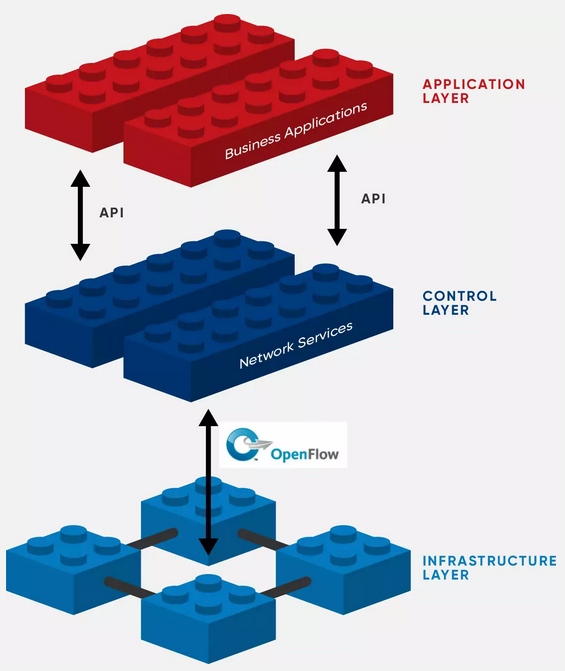
\includegraphics[scale=0.3]{openflow-basic.png}
\end{centering}

OpenFlow operates as TCP Protocol (6644 / 6653) and can be secured by TLS using certificates.

\noindent
Components of an OpenFlow Switch
\begin{itemize}
	\item Flow Table(s)
	\item Group Table
	\item OpenFlow channel(s) to external controller
\end{itemize}

\subsection{Controller}
OpenFlow messages -- for OF Channel setup between switch and controller:

\begin{table}[h]
	\begin{tabular}{l|l}
	HELLO & Sent by the switch, reply by the controller \\
		FEATURE\_REQUEST & Sent by controller, as supported OF capabilities \\
		FEATURE\_REPLY & Sent by switch to advertise \\
	\end{tabular}
\end{table}

Controller manages \emph{Flow Entries} in every switches flow tables (add, update, delete).

\subsection{Flow Tables}
Flow entry consists of
\begin{itemize}
	\item Match fields
	\item Counter
	\item Instructions
\end{itemize}

Replaces traditional MAC/CAM table that stores hosts' hardware addresses. A flow entry is selected by IP packet matching fields, first matching entry is used ordered by priority.
\begin{itemize}
	\item 39 fields possible to match on in OpenFlow 1.3, BUT must be supported by the hardware used
	\item usually in routing: most specific match
\end{itemize}

Instructions can be actions or modify pipeline processing. Possible actions are
\begin{itemize}
	\item Forward on port
	\item Drop
	\item Flood
	\item Send to controller
\end{itemize}

If no match in any flow table is found: TABLE\_MISS rule configuration: send to controller or drop.
